%! suppress = LineBreak
\documentclass[prd,twocolumn,tightenlines,preprintnumbers,showpacs,superscriptaddress,notitlepage,nofootinbib,eqsecnum,
floatfix,longbibliography]{revtex4-2}
\usepackage{CJK}
\usepackage[utf8]{inputenc}
\usepackage[T1]{fontenc}
\usepackage{amsmath}
\usepackage{mathtools}
\usepackage{amsfonts}
\usepackage{bm,bbm}
\usepackage{graphicx}
\usepackage{xcolor}

\usepackage{hyperref}
\hypersetup{
    colorlinks=true,       % false: boxed links; true: colored links
    linkcolor=blue,          % color of internal links
    citecolor=blue,        % color of links to bibliography
    filecolor=blue,      % color of file links
    urlcolor=blue           % color of external links
}

\begin{document}
\title{Solutions to Integer Programming from Quantum Annealing}

\author{Chia~Cheng~Chang (\begin{CJK*}{UTF8}{bsmi}張家丞\end{CJK*})}
\affiliation{RIKEN Interdisciplinary Theoretical and Mathematical Sciences (iTHEMS), Wako, Saitama 351-0198, Japan}
\affiliation{Department of Physics, University of California, Berkeley, California 94720, USA}
\affiliation{Nuclear Science Division, Lawrence Berkeley National Laboratory, Berkeley, California 94720, USA}
	\author{Chih-Chieh~Chen (\begin{CJK*}{UTF8}{bsmi}\mbox{陳志傑}\end{CJK*})}
\affiliation{R\&D Group, Grid Inc., Tokyo 107-0061, Japan}
\author{Christopher K\"orber}
\affiliation{Department of Physics, University of California, Berkeley, California 94720, USA}
\affiliation{Nuclear Science Division, Lawrence Berkeley National Laboratory, Berkeley, California 94720, USA}
\author{Travis~Humble}
\affiliation{Quantum Computing Institute, Oak Ridge National Laboratory, Oak Ridge, Tennessee 37831, USA}
\author{Jim~Ostrowski}
\affiliation{University of Tennessee}

\begin{abstract}
Abstract here...
\end{abstract}

\preprint{RIKEN-iTHEMS-Report-20}

\maketitle
%%%%%%%%%%%%%%%%%%%%%%%%%%%%%%%%%
%%%%%%%%%%%%%%%%%%%%%%%%%%%%%%%%%
%%%%%%%%%%%%%%%%%%%%%%%%%%%%%%%%%
%\tableofcontents

\flushbottom
\maketitle

\section{INTRODUCTION}
\label{sec:introduction}

Integer linear programming (ILP) is an integer optimization problem subject to inequality constraints and is a commonly tackled problem applicable to situations such as x~\cite{}, y~\cite{}, and z~\cite{}. In general however, ILP is classically NP-complete, and as a result, heuristic methods are employed~\cite{}. The NP-hardness of ILP can be understood by realizing that while the solution to an $n$-dimensional linear problem can be obtained in polynomial time, the optimal integer solution in general must be found in the $2^n$ integer solutions which surround the real number solution. Due to the importance and difficulty, in this work we present a method to obtain the optimal solution to ILP by employing methods of quantum annealing.

Quantum annealing solves a general quadratic binary optimization problem (QUBO) by slowly varying a time-dependent Hamiltonian~\cite{}. Through the adiabatic theorem of quantum mechanics, the annealer is prepared initially in a trivial ground state while the solution to ILP is encoded in the target Hamiltonian. Due to the explosion in research efforts towards hardware implementations of quantum annealers and future improvements to the annealing schedule~\cite{}, mapping ILP to QUBO provides a path forward towards obtaining optimal solutions to the class of integer optimization problems~\cite{2018Glover}.

Formally, ILP is defined as the optimization of a linear function
\begin{align}
f(x) = &\min\limits_{x}(\sum_i c_i x_i),\\
\textrm{subject to } &\left \{
\begin{matrix*}[l]
	&\sum_i A_{ai}x_i +b_a \leq 0 \\
	&x_i \geq 0,\\
	&x_i \in \mathbb{Z}
\end{matrix*} \right.
\end{align}
where $i=1, \cdots,  N$ is the number of dependent variables and $a=1, \cdots, M$ the number of constraint equations. The inequality constraints can be rewritten as an equality by introducing slack variables $s$ such that the ILP becomes
\begin{align}
f(x) = &\min(\sum_i c_i x_i),\\
\textrm{subject to } &\left \{
\begin{matrix*}[l]
	&\sum_i A_{a i}x_i + s_a + b_a = 0,\\
	&s_a \geq 0,\\
	&s_a \in \mathbb{Z},\\
	&x_i \geq 0,\\
	&x_i \in \mathbb{Z}.
\end{matrix*} \right.
\end{align}
Since quantum annealing solves the QUBO problem, we extend the proposed algorithm to solve integer quadratic optimization problems such that
\begin{align}
f(x) = \min\limits_{x}\left(\sum_{ij} x_i d_{ij} x_j + \sum_i c_i x_i\right)
\end{align}
without the introduction of auxiliary qubits.


\section{RESULTS}
\label{sec:results}
We map integer variables $z_i$ to qubits under the following transformation~\cite{Chang:2018uoc}
\begin{align}
z_i = & \sum_{r=0}^{R_i-1} 2^r \psi_{ri}
\label{eq:int_to_bin}
\end{align}
where $\psi_{ri} \in \{0, 1\}$ while the number of qubits used to represent the $i$-th integer variable is allowed to vary with $R_i$. The transformation can in general be express as a rectangular matrix. For example, a vector of two integer variables $z_0$ and $z_1$ represented by one and two qubits respectively is given as
\begin{align}
\begin{pmatrix}
z_0\\
z_1
\end{pmatrix}
= &
\begin{pmatrix}
2^0 & 0 & 0\\
0 & 2^0 & 2^1
\end{pmatrix}
\begin{pmatrix}
\psi_{00}\\
\psi_{01}\\
\psi_{11}
\end{pmatrix}
\equiv T^z \begin{pmatrix}
\psi_{00}\\
\psi_{01}\\
\psi_{11}
\end{pmatrix}
\end{align}
The transformation can be reduced to a tensor product if $R_i$ is a constant for all $i$ such that
\begin{align}
\mathcal{R} = & \begin{pmatrix} 2^0 & \dots & 2^{R-1}\end{pmatrix},\\
\mathcal{Z} = & \begin{pmatrix} z_0 & \dots & z_{N-1}\end{pmatrix},\\
|\mathds{1}| = & |\mathcal{Z}|,\\
T^z = & \mathds{1}\otimes \mathcal{R}.
\end{align}

While the coefficients of the inequality constraints are not required to be integer valued, the inequalities can be trivially rescaled such that $s_i \in \mathbb{Z}$ given fixed precision coefficients $A_{ij}$ and $b_i$. As a result, we can restrict both $x_i$ and $s_i$ to sample over only positive integer values as allowed by Eq.~(\ref{eq:int_to_bin}).

\subsection{Integer Programming Mapping to QUBO}
\label{sec:results:ilp}
The integer quadratic optimization problem can be mapped to a minimization of the quadratic objective function
\begin{align}
\chi^2 = & \left[\Psi^x_{\mu} T^x_{\mu i}d_{ij} T^x_{j \nu}\Psi^x_\nu + c_i T^x_{i\mu} \Psi^x_\mu \right. \nonumber\\
&\left.+ p (A_{a b} T^x_{b \mu} \Psi^x_{\mu} + T^s_{a \alpha} \Psi^s_\alpha + b_a)^2 \right],\\
\Psi = & \begin{pmatrix}
\Psi^x\\
\Psi^s
\end{pmatrix},
\end{align}
where $p$ is the strength of the penalty factor which must be set large enough such that the constraints are satisfied under minimization. The objective function can be represented as a QUBO Hamiltonian
\begin{align}
E = &
\begin{pmatrix}
\Psi^x & \Psi^s
\end{pmatrix}
\begin{pmatrix}
Q_{xx} & Q_{xs}\\
Q_{sx} & Q_{ss} 
\end{pmatrix}
\begin{pmatrix}
\Psi^x\\ \Psi^s
\end{pmatrix} + pb^2,\\
\equiv & \Psi^T Q \Psi + C,
\label{eq:matrix_form}
\end{align}
where
\begin{align}
Q_{xx} = & {T^{x}}^T \left[ d + p A^T A + p \mathrm{Diag}_{x} \left(A^T b + b^T A\right) \right] T^x \nonumber \\
&+ \mathrm{Diag}_{\psi^x}(c) T^x,\\
Q_{xs} = & Q_{sx}^T = p {T^{x}}^T A^T T^s,\\
Q_{ss} = & p\left[ {T^{s}}^T T^s + \mathrm{Diag}_{\psi^s}\left( {T^{s}}^T b + b^T T^s\right) \right].
\end{align}
The function $\mathrm{Diag}_{z}(v)$ embeds a vector $v$ into a diagonal matrix in subspace $z$, and absorbs the linear contributions of the QUBO into the diagonal elements of the quadratic representation.

\subsection{Application to the Dominating Set Problem}
\label{sec:results:mds}

Given a graph $G(E,V)$, defined by the set of $V$ vertices and $E$ edges, and a subset of vertices $D \subseteq V$. If the set of all vertices not in $D$ is adjacent to at least one vertex in $D$, then $D$ is a dominating set. This is equivalent to requiring the set of nearest-neighbor vertices of $D$ (exclusive) and $D$ cover all vertices $N(D) \cup D = V$ (an example is given by Fig.~\ref{fig:dominating_sets}a). The set $D$ is a minimal dominating set if there is no proper subset of $D$ that is a dominating set, {\it{i.e.}}, the removal of any vertex in $D$ results in $N(D) \cup D  \neq V$. An example is given by Fig.~\ref{fig:dominating_sets}b. The domination number of $D$ is given by the cardinality of $|D| \equiv \overline{\overline{D}}$. The minimum dominating set (MDS) is defined by $D$ with the smallest domination number. Fig.~\ref{fig:dominating_sets}c shows an example of the minimum dominating set of $G(V, E)$ and is different from the minimal dominating set. We emphasize that while the maximum independent set is always a minimal dominating set as exemplified by Fig.~\ref{fig:dominating_sets}b, the minimum dominating set in general can have a smaller domination number. As a result, the solution to the dominating set problem can not be obtained by solving for the maximum independent set, a problem that is well studied for quantum annealers~\cite{}.

\begin{figure*}
	\centering
	\begin{tabular}{p{0.2\textwidth}p{0.1\textwidth}p{0.2\textwidth}p{0.1\textwidth}p{0.2\textwidth}}
	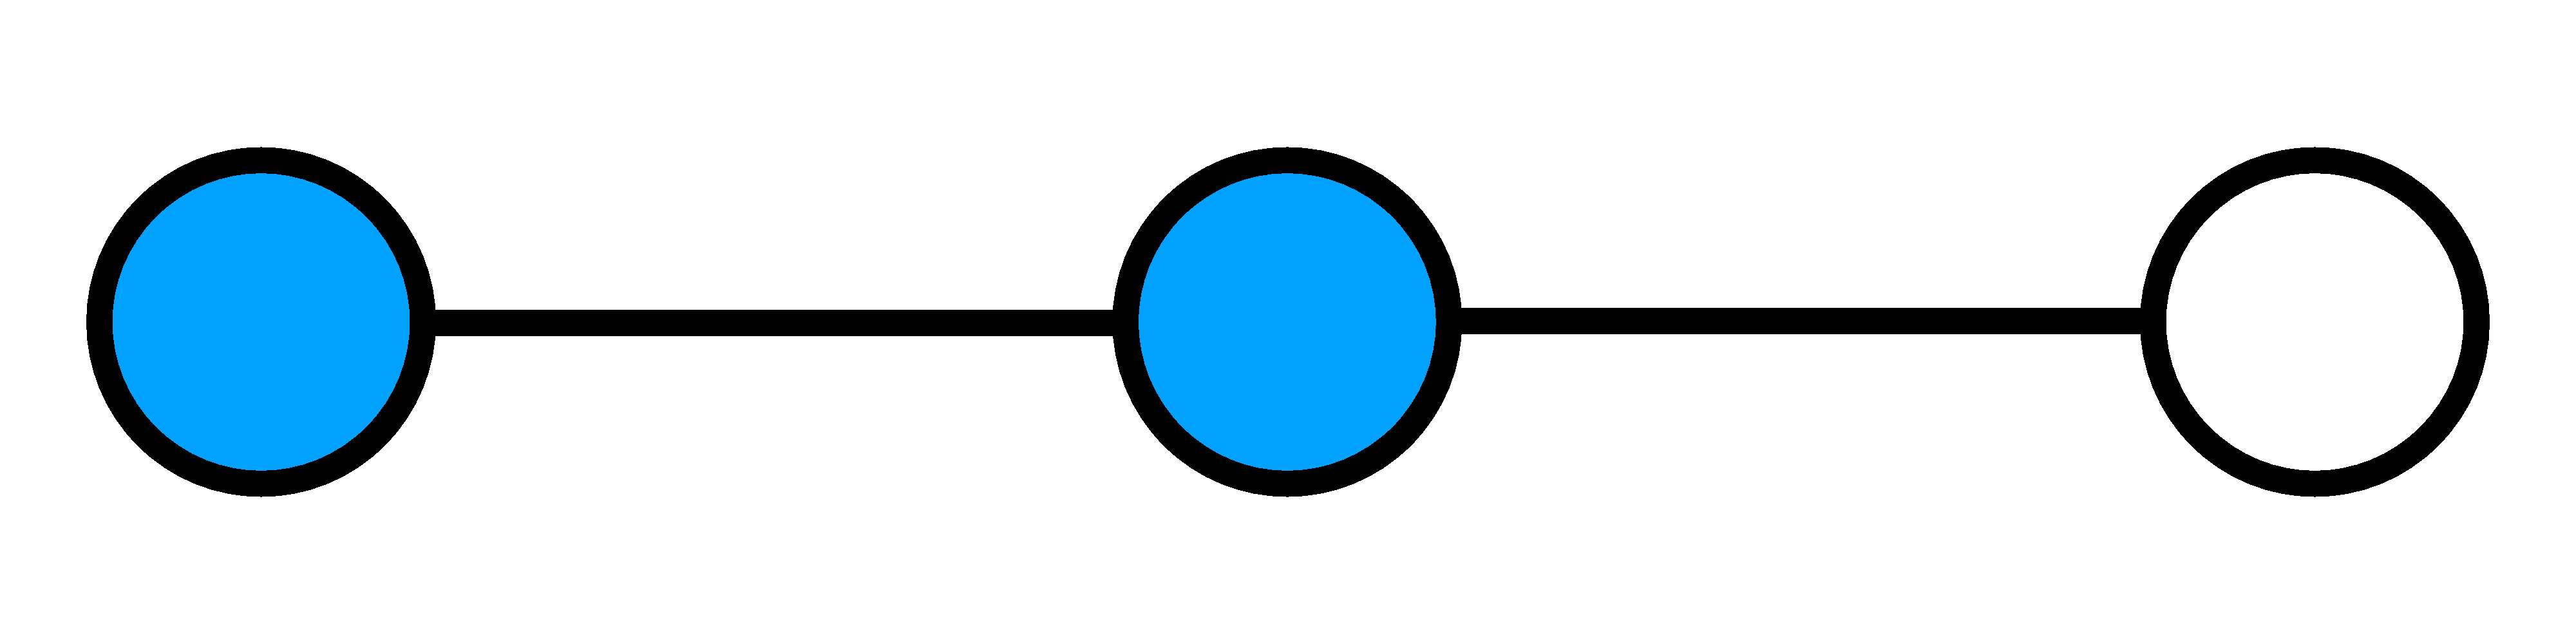
\includegraphics[width=0.2\textwidth]{./new_figures/MDS_mds0.pdf}
&&
	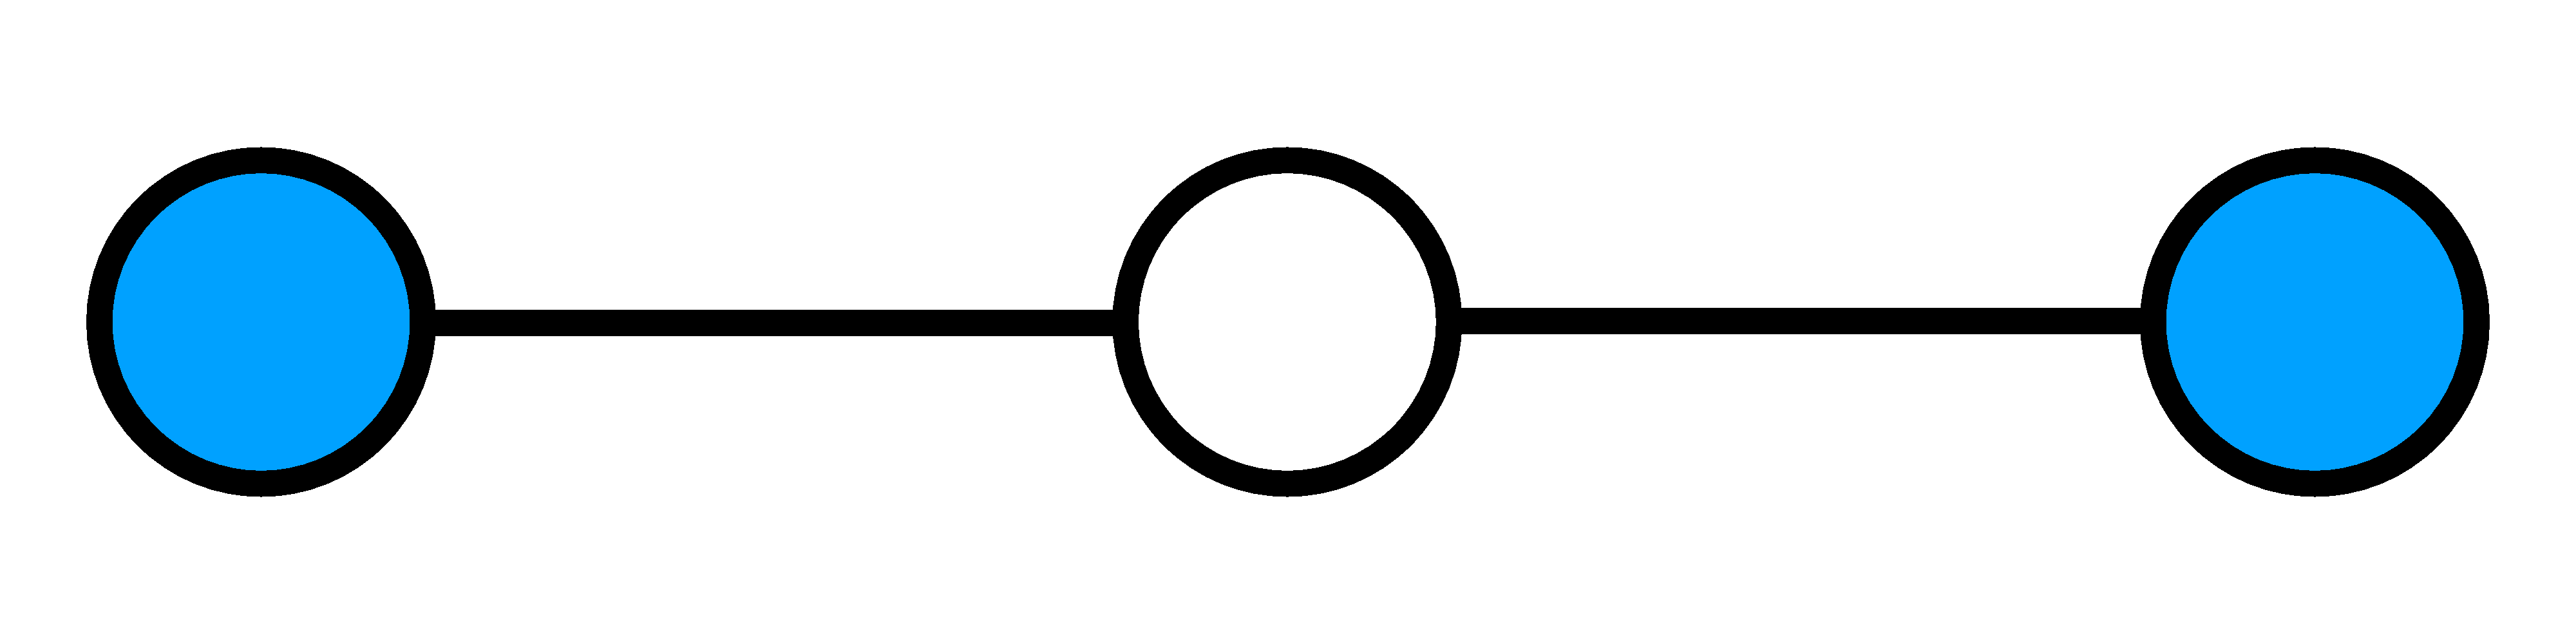
\includegraphics[width=0.2\textwidth]{./new_figures/MDS_mds1.pdf}
&&
	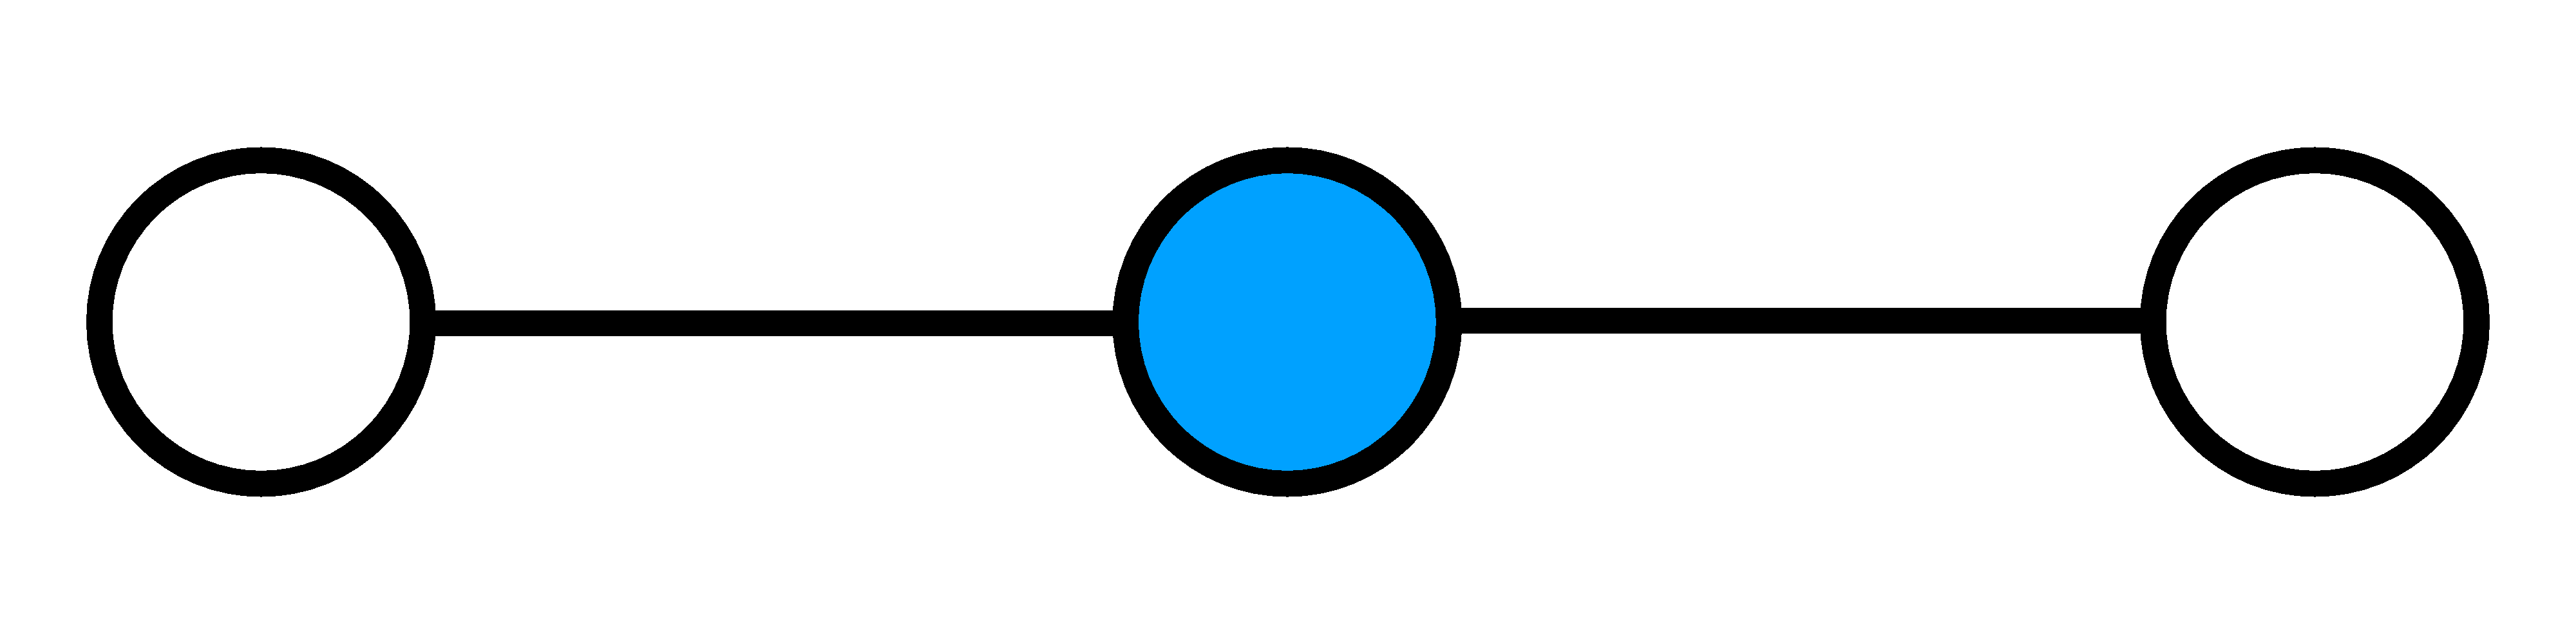
\includegraphics[width=0.2\textwidth]{./new_figures/MDS_mds2.pdf}\\
	\centering\bf{a} && \centering\bf{b} && \centering\bf{c}
	\end{tabular}
	\caption{Example of different dominating sets for $G(V, E)$. Vertices in the dominating set $D$ are highlighted in blue. {\bf{a)}} A dominating set of $G$ with domination number $\overline{\overline{D}} = 2$. {\bf{b)}} A minimal dominating set of $G$ with domination number of $\overline{\overline{D}} = 2$. {\bf{c)}} The minimum dominating set of $G$ with domination number of $\overline{\overline{D}} = 1$.}
	\label{fig:dominating_sets}
\end{figure*}

For general graphs, existing "classical" algorithms either find minimal solutions in exponential time $\sim O( 1.5^n)$ \cite{Fomin2009, vanRooij2009} or approximate solutions in polynomial time. For example, greedy algorithms locally optimize decisions about which nodes to add to the dominating set.
Thus one is guaranteed to find a dominating set but not necessarily a MDS. {\color{red} Write some pseudo code for greedy search.}
%We demonstrate an example greedy algorithm in figure Fig.~\ref{fig:mds-greedy}.

\iffalse
\begin{figure*}
	\centering
	\begin{tabular}{p{0.22\textwidth}p{0.22\textwidth}p{0.22\textwidth}p{0.22\textwidth}}
	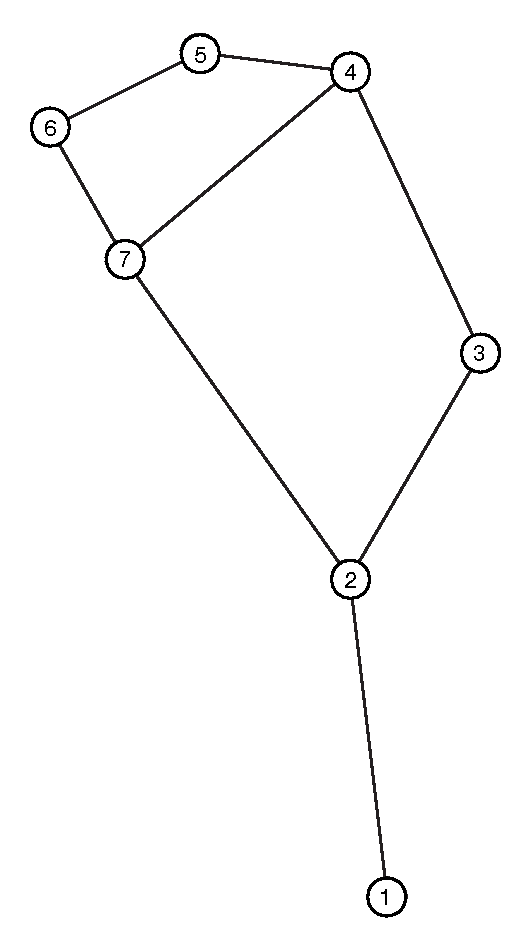
\includegraphics[width=0.20\textwidth]{./figures/greedy-1.pdf}
&
	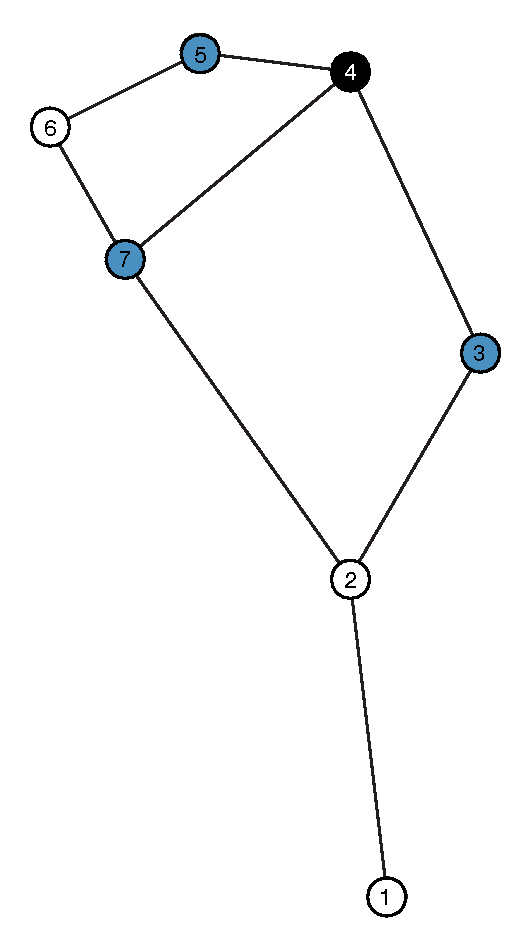
\includegraphics[width=0.20\textwidth]{./figures/greedy-2.pdf}
&
	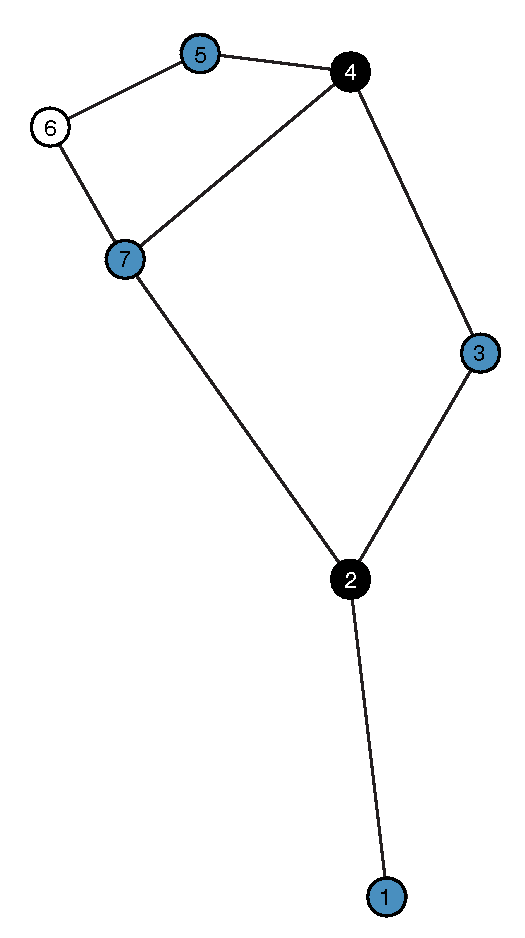
\includegraphics[width=0.20\textwidth]{./figures/greedy-3.pdf}
&
	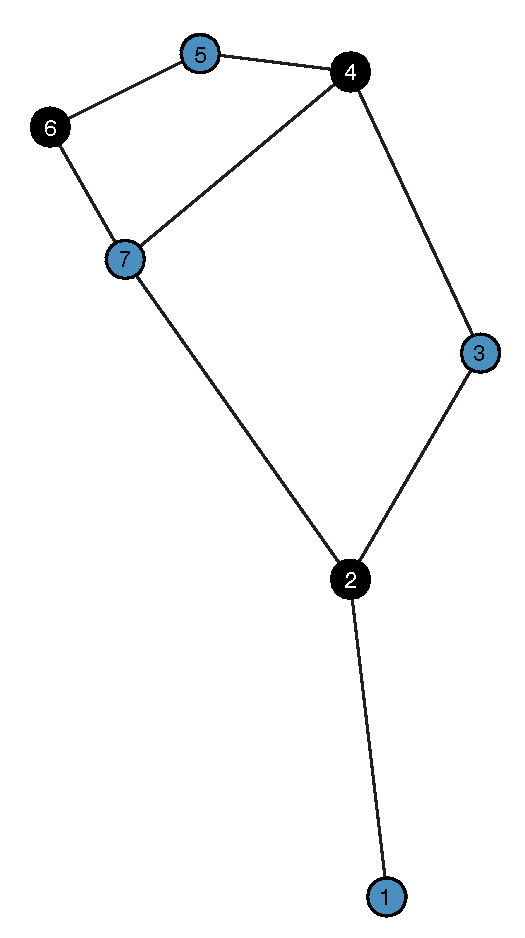
\includegraphics[width=0.20\textwidth]{./figures/greedy-4.pdf}\\
	\centering\bf{a} & \centering\bf{b} & \centering\bf{c} & \centering\bf{d}
	\end{tabular}
	\caption{
		Example of greedy MDS algorithm:
		The algorithm iteratively adds vertices to the dominating set (black nodes) such that newly added nodes are maximally unconnected (white nodes).
		Connected nodes are neighbors of the DS (turquoise) or already in the DS.
		In (a), one finds three unconnected nodes [(2), (4), (7)] which are adjacent to three unconnected nodes each.
		In the first step $a\to b$, randomly the node (4) is picked.
		In (b), one has two unconnected choices [(1), (2)] with each adjacent to another unconnected node.
		After randomly selecting (2) when going from $b \to c$, only one unconnected node is remaining (6).
		The found solution is a (minimal) dominating set but not a MDS.
		To find the MDS using this greedy algorithm, the first node choice must be either (2) or (5).
	}
	\label{fig:mds-greedy}
\end{figure*}
\fi

\subsubsection{Minimum Dominating Set}
The solution to the minimum independent set can be expressed as an integer optimization problem given by,
\begin{align}
f(x) = &\min(\sum_{\nu \in V} \psi^x_{\nu}),\\
\textrm{subject to} \quad & \psi^x_{\nu} + \sum_{\mu \in \mathit{N}(\nu)} \psi^x_{\mu} \geq 1,\\
& \psi^x_{\nu} \in \{0, 1\}
\end{align}
where the dimension of the dependent variable $x$ is the number of vertices $\overline{\overline{V}}$.
The problem minimizes the number of vertices in $D$ with a binary variable $\psi^x$ encoded by a single qubit, subject to the constraint that at least one vertex in $\mathit{N}(\nu)$ is in $D$. For each vertex in $V$ we introduce slack variables $s_{\nu} = T^s_{\nu \alpha} \psi^s_{\alpha}$ to encode the inequality constraint such that
\begin{align}
f(x) = &\min(\sum_{\nu\in V} \psi^x_{\nu}),\\
\textrm{subject to} \quad & \psi^x_{\nu} + J_{\nu \mu} \psi^x_{\mu}- T^s_{\nu \alpha} \psi^s_{\alpha}  - 1 = 0,\\
& \psi_{\nu} \in \{0, 1\},\\
& 0 \leq s_{\nu} \leq |\mathrm{N}(\nu)|\\
& s_{\nu} \in \mathbb{Z},
\end{align}
where the nearest-neighbor sum is expressed by $J$ (symmetric and zero diagonal), the adjacency matrix for $G$.
The algorithm uses $N_q = \overline{\overline{V}} + \sum_{\nu \in V} \log_2 \mathit(N(\nu))$ qubits---$\overline{\overline{V}}$ qubits to encode the vertices and another $\sum_{\nu \in V} \log_2 \mathit(N(\nu))$ qubits to embed the slack variables. Therefore, the embedding at worse scales with $\overline{\overline{V}} \log_2 |\overline{\overline{V}}|$ qubits for fully connected graphs.

The target Hamiltonian can be written in the matrix form
\begin{widetext}
\begin{align}
E = &
\begin{pmatrix}
\Psi^x & \Psi^s
\end{pmatrix}
\begin{pmatrix}
\mathbbm{1} + p\left[J^T J + J^T + J - 2 \mathrm{Diag}_{\psi^x}(|J|) - \mathbbm{1} \right] & - p(\mathbbm{1}+J^T)T^s\\
- p{T^s}^T(\mathbbm{1}+J)& p\left[{T^s}^T T^s + 2\mathrm{Diag}_{\psi^s}(|T^s|)\right]
\end{pmatrix}
\begin{pmatrix}
\Psi^x\\ \Psi^s
\end{pmatrix} + p \overline{\overline{V}}
\label{eq:matrix_form2}
\end{align}
\end{widetext}
where $ |M| \equiv \sum_{\nu} M_{\nu \mu}$.

\section{DISCUSSION}

\subsection{Finding the Dominating Set with a Quantum Annealer}
\label{sec:discussion:qa}
\begin{figure}[b]
	\centering
	\begin{tabular}{cc}
	$G(n):$ &
	\raisebox{-.4\height}{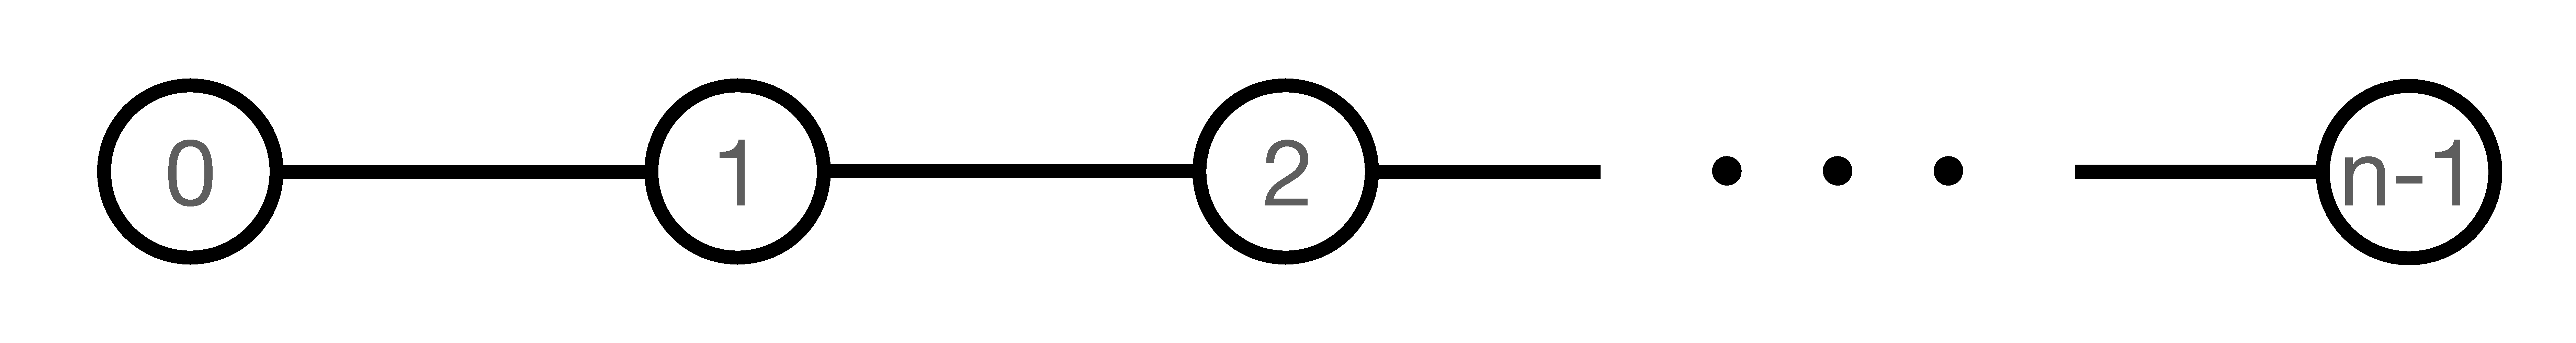
\includegraphics[width=0.8\columnwidth]{./new_figures/linear_graph.pdf}}
	\end{tabular}
	\caption{Linear graphs $G(n)$ used in this study. Nodes denote vertices of the graphs and lines are undirected edges.}
\label{fig:linear}
\end{figure}

We demonstrate the proposed algorithm in order to obtain the MDS on a series of linear graphs $G(n)$ as shown in Fig.~\ref{fig:linear}. This type of graph is chosen because the small number of nearest-neighbor connections is more efficiently embedded into the chimera graph allowing for scaling plots to be generated when using a DWave quantum annealer. Additionally the MDS solution is known analytically, and contains both unique and degenerate solutions. In particular, the domination number for $G(n)$ is $\lceil n/3 \rceil$ while the number of MDS solutions for $n$ vertices is
\begin{align}
&1 &&\textrm{if} && n\textrm{ mod }3=0,\nonumber \\
&2\lfloor n/3 \rfloor + 1 && \textrm{if}&& n\textrm{ mod }3=1,\nonumber \\
&\lfloor n/3 \rfloor + 2 && \textrm{if} && n \textrm{ mod }3 = 2,
\end{align}
and gives the probability of randomly guessing the MDS of $G(n)$.

For the following studies, we perform experiments on the \texttt{DW\_2000Q\_6} solver. The annealing time is set to 500$\mu$s after performing a study on various annealing times the $G(6)$ graph. The black line (offset$=0.0$) in Fig.~\ref{fig:baseline} shows results from the baseline experiment, without modification to the DWave annealing schedule, and observe improvement over random guessing (blue). However, We explore one avenue towards improving the experiment results by introducing per-qubit annealing offsets into the time evolution.

\begin{figure}
	\centering
	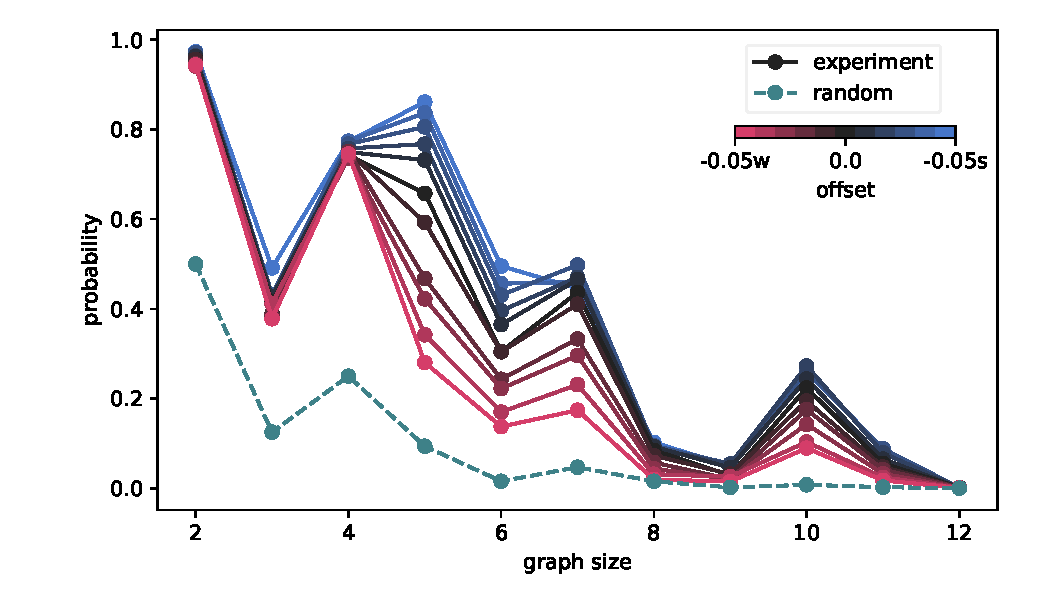
\includegraphics[width=\columnwidth]{./new_figures/DWave_scaling.pdf}
	\caption{Baseline result of DWave (black) compared to random guessing (blue). The jagged nature of random guessing reflects the degeneracy of the ground state. The legend labels the values of annealing offsets employed. A positive offsets (yellow) indicates that qubits with large values of $|h_i|$ are annealing with a delayed schedule, while negative offsets (green) delay the schedule of qubits with small values of $h_i$.}
	\label{fig:baseline}
\end{figure}

\subsubsection{Modified annealing schedule}

\noindent\textit{Annealing offsets}

In quantum annealing, the ground state of the problem Hamiltonian is obtained from the evolution of a time-dependent Hamiltonian,
\begin{equation}
H(s) = A(s) H^{\textrm{init}} + B(s) H^{\textrm{problem}}, \label{eq:tdhamiltonian}
\end{equation}
where $H^\textrm{init}=\sum_i\sigma^x_i$ on the DWave, and $H^\textrm{problem}$ is given by Eq.~(\ref{eq:matrix_form}) for the MDS application. The variable $s\in [0, 1]$ is the normalized annealing time and is allowed to vary between 1$\mu s$ to 2$ms$ on the DWave. On DWave solvers, annealing offsets effectively advance or delay the annealing schedule of individual qubits. In Fig.~\ref{fig:anneal_schedule}, the default DWave annealing schedule is shown in black, in addition to the effects of applying negative offsets (effective time delay) to $A(s)$ and $B(s)$ in blue. The time dependent coefficients are nonlinear in time because the underlying control variable $c(s)$ which is designed to grow the persistent current $I_p(s)$ linearly in time. The effective time delay is implemented by introducing an offset as $c(s) + \delta$.  As a result, systematic errors are introduced because the final values of $A(s)$ and $B(s)$ will differ for qubits with different offsets. Additionally, the values of the coefficients are unknown outside of $s\in [0, 1]$. We extrapolate their values by a linear extrapolation, and only employ negative offsets such that this effect only enters at the beginning of the annealing process rather than the end. Details of the DWave annealing schedule use to generate Fig.~\ref{fig:anneal_schedule} and further documentation are provided by DWave in Ref.~\cite{dwave_as, dwave_as_docu}.

\begin{figure}[b]
	\centering
	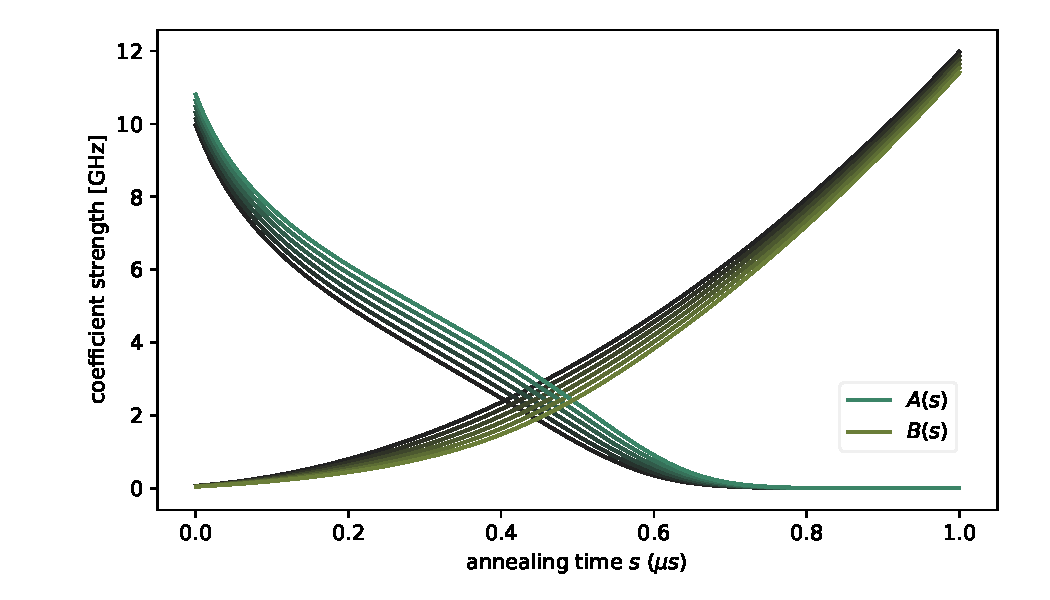
\includegraphics[width=\columnwidth]{./new_figures/anneal_schedule.pdf}
	\caption{asdf}
	\label{fig:anneal_schedule}
\end{figure}

The motivation behind implementing per-qubit level offsets is rooted in the hypothesis that as the problem Hamiltonian is turned on, the system in general will exhibit more disorder. We define disorder by first recasting the QUBO into its Ising form such that the problem Hamiltonian has the form
\begin{equation}
H^{\textrm{Ising}} = \sum_{ij} J_{ij} \sigma^z_i \sigma^z_j + \sum_i h_i \sigma^z_i,
\end{equation}
and recognize that in the limit where $h_i$ is randomly drawn from a Bernoulli distribution we recover the spin-glass model. The spin-glass model enters its glassy state when $|h_i|$ is large, and as a consequence, the wavefunction experiences many-body localization effects, the many-body analogue of Anderson Localization (MBL)~{\color{red} cite some AL papers here}.
\\\\
\noindent\textit{Implementation of annealing offsets}
\label{sec:discussion:offsets}

For even the smallest graph $NN(2)$, the MDS problem is not native to the chimera graph and must be embedded. Following the hypothesis of MBL, we therefore, must look at the values of $h_i$ after embedding. The qubits then split into two groups depending on the value of $h_i$ relative to $(\textrm{max}|\{h\}| - \textrm{min}|\{h\}|) / 2$ given the set of external magnetic fields $\{h\}$ defined by a specific embedding. Further detail is given in Sec.~\ref{sec:methods:minor_embedding} {\color{red} put in methods more details}. We study the effects offset the two groups of qubits over a total range between 0\% and 5\% of $c$. The results of this study is shown in Fig.~\ref{fig:dwave_offset}.

The results in yellow (green) delays the annealing of qubits subject to stronger (weaker) external fields. We observe improvement (diminishment) in the experimental results when qubits subject to stronger (weaker) final external fields are delayed in the anneal schedule, in agreement with the MBL hypothesis. The phenomena is observed across different problem sizes and hints at the possibility of a generic improvement strategy. In the following section, we provide evidence that the improvement is rooted in quantum mechanics, and not other causes such as imperfections in hardware~\cite{} {\color{red} cite dwave's use of annealing offsets}. The master equation for quantum annealing is solved subject to the DWave anneal schedule with annealing offsets in order to reproduce the observed phenomenon.

\subsection{Simulation Results}

In order to understand the effects of annealing offsets, we simulate the annealing process for the $G(2)$ graph embedded in chimera topography. In order to shorten the simulation time, we resample the DWave with a total annealing time of 1 $\mu s$. The resulting ground state probability as a function of offset measured over 100,000 observations is shown in Fig.~\ref{fig:dwave1us}.

\begin{figure}
	\centering
	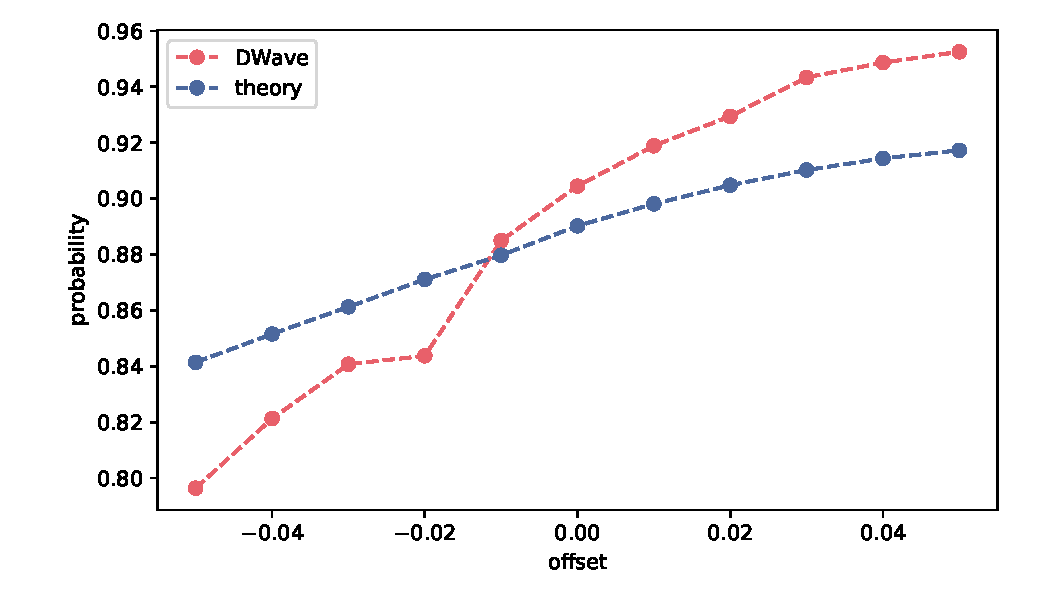
\includegraphics[width=\columnwidth]{./new_figures/NN2_offset_scaling.pdf}
	\caption{ {\color{red} new caption}}
	\label{fig:dwave1us}
\end{figure}

Simulation results are obtained by solving the von Neumann equation subject to two decoherence models: local damping and full-counting statistics. Details of the master equation are given in Sec.~\ref{sec:methods:lindblad}. The time dependence of $A(s)$ and $B(s)$ are given by the DWave annealing schedule with offsets in Fig.~\ref{fig:anneal_schedule}. The graph $G(2)$ has the interesting feature of having a degenerate ground state depending on whether qubit 0 or 1 is chosen to be the MDS solution. This degeneracy is reflected in the experimental result and provides a non-trivial benchmark for our simulation. Fig.~\ref{fig:final_state_distribution} show the final state distribution of the three lowest lying state. The states $(0, 1, 0, 0, 0)$ and $(1, 0, 0, 1, 0)$ are the two degenerate ground states of the embedded Hamiltonian, while $(1, 1, 1, 1, 1)$ is the first excited state which yields an incorrect solution. All other states receive negligible probability at the end of annealing. The simulation (black) captures main features of the experimental result: 1) significant probability to populate both ground states (rather than populating only one), 2) asymmetry in ground state population due to systematic effects of offset lifting the final state degeneracy spanning approximately the correct range, 3) population of first excited state with systematically lower probability when the strong field is delayed. This result can be obtained by tuning three free parameters: the simulation temperature to the order of 10 milliKelvin, and the two coefficients of the two decoherence models at the order of 1 to 10 $ns$. Additional insights of the simulation are given in Sec.~\ref{sec:methods:simulation_details}.

The resulting probability of recovering the correct solution as a function of annealing offset is given in Fig.~\ref{fig:dwave1us}. We confirm that scaling with respect to offset from the simulation matches what is observed from experiment. Furthermore, in Sec.~\ref{}, we provide the results of an ideal quantum annealer, where the annealing schedule is faithfully delayed (all qubits start and end with the same values of $A$ and $B$) and all decoherence terms are removed. The scaling with respect to offset is preserved indicating that the improvements are related to quantum mechanics.

\begin{figure}
	\centering
	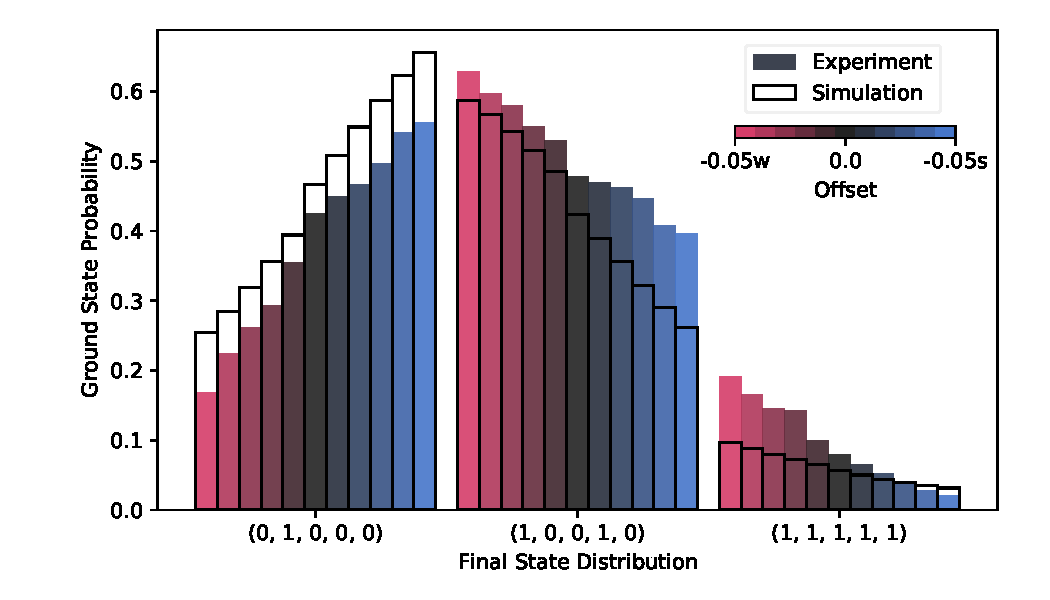
\includegraphics[width=\columnwidth]{./new_figures/final_state_distribution.pdf}
	\caption{{\color{red}I need to add dwave final state distribution here too.}}
	\label{fig:final_state_distribution}
\end{figure}

\subsection{Final remarks}
We would like to emphasize that while the annealing offsets are motivated by the MBL hypothesis, and the results also follow those expectations, we do not have definitive proof that MBL plays a crucial role. The reason is because observations of MBL inevitably require the study of finite-size scaling, and our current simulation while being extremely thorough and explicit, is exponentially slow to evaluate making evaluations of even $G(3)$ untenable. However, the intersection of time-dependent quantum mechanics and emergent phenomena such at MBL is an exciting direction that is pertinent to adiabatic quantum computing.


\section{METHODS}
\subsection{The Lindblad Equation}
\label{sec:methods:lindblad}

To solve for time evolution dynamics of quantum annealing including thermal and the decoherence effects, we solve for the master equation in Lindblad form
\begin{align}
\partial_t \rho (t) =  \frac{-i}{\hbar} [H(t) , \rho(t)] + \mathcal{L}[\rho (t)] ,
\end{align}
where $\rho (t)$ is the density matrix at time $t$. $H(t)$ is the time-dependent Hamiltonian 
\begin{align}
\label{eq:annealH}
 H_{anneal}(t)&  =  - \sum_i  A_i(t)\sigma^x_i & \notag \\ 
 +&  \sum_{i>j} \sqrt{B_{i}(t)B_{j}(t)} J_{ij} \sigma^z_i \sigma^z_j +\sum_i B_{i}(t) h_i \sigma^z_i  ,&
\end{align}
where $A_i(t)$ and $B_{i}(t)$ are site-dependent annealing schedule functions. The site dependency takes into account of the annealing offset. $[,]$ denotes the Lie bracket and $\mathcal{L}$ is the Lindblad operator.

We consider two types of decoherence models: full counting statistics and local damping. The full counting statistics term models the global decoherence to all the qubits due to the classical reservoir. The local damping term models the decoherence of each qubit independently. 
For full counting statistics, the Lindblad operator is 
\begin{align}
\mathcal{L}[\rho (t)] &=& \Gamma_{fc} \sum_j   (2 S_j \rho(t) S_j^\dagger - \{ S^\dagger_j S_j, \rho(t) \}) \notag \\
&& + e^{-\beta \Delta E_j} (2 S_j^\dagger \rho(t) S_j - \{ S_j S^\dagger_j, \rho(t) \} )
\end{align}
where $j$ is the index for the inter-level spacing $\Delta E_j=E_\mu-E_\nu>0$. $S_j=|E_\nu \rangle \langle E_\mu|$ denotes the many-body lowering operator. $\{, \}$ denotes the anti-commutator. $\Gamma = 1/T_c$ is the decoherence rate for coherence time $T_c$. That is, due to the interaction with the classical thermal bath, there is a probability that the system hops from each higher-energy many-body state to a lower-energy many-body state. The probability of the inverse process is given by a Boltzmann factor. To model the local decoherence of each qubits in the non-interacting limit, we also consider the amplitude damping for non-interacting qubits. The Lindblad operator is 
\begin{align}
\mathcal{L}[\rho (t)] &=&  \Gamma_{loc} \sum_j (2L_j \rho(t) L_j^\dagger - \{ L^\dagger_j L_j, \rho(t) \} \notag \\
&& + e^{-\beta 2|h_j| }  (2L_j^\dagger \rho(t) L_j - \{ L_j L_j^\dagger, \rho(t) \}) ),
\end{align}
where $j$ is the index for qubit. $L_j= \sigma^{+}_j=|1\rangle \langle 0|$ for $h_j>0$ and $L_j= \sigma^{-}_j=|0\rangle \langle 1|$ for $h_j<0$. That is, each qubit is damped toward its local ground state if we ignore all the interactions. 

The initial condition is the Gibbs canonical ensemble
\begin{equation}
\rho (0) =  \frac{e^{-\beta H(0)}}{\mbox{Tr}[e^{-\beta H(0)}]} ,
\end{equation}
where $\beta$ is the inverse temperature.
The probability to get the ground state at measurement is
\begin{align}
P =  \mbox{Tr} \{  \rho (t) \pi_{\mbox{gnd}} \}  ,
\end{align}
where the projection operator onto the degenerated ground states subspace is defined as $\pi_{\mbox{gnd}}=\sum_{i\in G} |\mbox{gnd}_i\rangle \langle \mbox{gnd}_i| $. Here $\{ | \mbox{gnd}_i \rangle | i \in G \}$ forms an orthonormal basis for the degenerated ground states subspace, i.e., $\langle \mbox{gnd}_j | \mbox{gnd}_i \rangle = \delta_{ij}$.

\subsection{Minor Embedding}
\label{sec:methods:minor_embedding}
Our proposed offset strategy is motivated by the structure of the Hamiltonian being evaluated by the annealer. As a result, details of the embedding are important. We obtain an embedding for $G(n)$ with the \texttt{embed\_qubo} function provided by the DWave Oceans Python package~\cite{dwave_oceans} under the \texttt{dwave.embedding} module. The same embedding is used for all DWave solves of the same graph (independent of offset), and consequently the simulation solves the resulting embedded Hamiltonian for $G(2)$. Additionally, solving the same graph as a function of offset on the exact same qubits removes (or at least keeps consistent) the systematic effects due to solving a problem on different physical qubits. We note that comparisons between different graphs in Fig.~\ref{fig:baseline} are subject to this uncontrolled systematic.

After embedding the QUBO for $G(2)$ requires 5 qubits (an increase from 4), where by construction, qubits 0 and 3 form the qubit chain. We confirm through brute force evaluation of the eigenvalue decomposition of the 5 qubit Hamiltonian, that the embedding provided by DWave solves the expected ILP problem for $G(2)$, with degenerate ground states at $(0, 1, 0, 0, 0)$ and $(1, 0, 0, 1, 0)$ corresponding to whether vertex 0 or 1 is chosen for the MDS solution, and $(1, 1, 1, 1, 1)$ as the first (non-degenerate) excited state where both vertex 1 and 0 are in the set yielding a valid dominating set but not the minimum dominating set.

The resulting Ising Hamiltonian has external field equal to $h = (2.75, 1.5, -1.0, -1.25, -1.0)$. Following the offset strategy described in Sec.~\ref{sec:discussion:offsets}, qubit(s) 0 (1, 2, 3, 4) are placed in the set with relatively stronger (weaker) final external fields. This imbalance in the two groups may perhaps explain the reason why effects of delaying the weaker fields are more pronounced, since delaying the strong fields only differs from the baseline by a single qubit.

\subsection{Simulation Details}
\label{sec:methods:simulation_details}
To check the correctness of simulator and unit conversion, we tested a simple annealing schedule for pure transverse field, i.e. $A(s)=A(0)$ and $B(s)=0$. The initial state is pure zero state $\rho=|00...0\rangle \langle 00...0|$. In this case the analytical solution can be obtained for the wave function oscillation. The time-dependent probability is $P_{0}=\cos^{2n}(s)=\cos^{2n}(t/T)$ where $n$ is the number of qubits and $T$ is the annealing time. For annealing time $T=1/A(0)$, we expect to see perfect one-period oscillation. The energy spectrum for this system can be analytically obtained, so we also checked the Boltzmann distribution in the initial density matrix construction. {\color{red} Are you suppose to reference Fig. 7 here?}

\begin{figure}
	\centering
	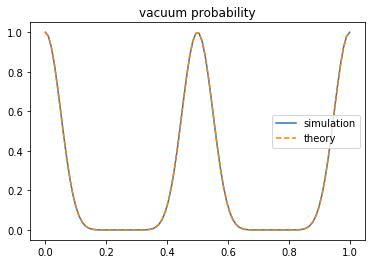
\includegraphics[width=\columnwidth]{./figures/check.png}
	\caption{check}
	\label{fig:check}
\end{figure}

Next, the simulator is applied to the $G(2)$ problem and the result is summarized in Fig.~\ref{fig:td_prob} where the time-dependent overlap with the exact Ising ground state is shown. We observe for all cases that the system undergoes what is analogous to a magnetic phase transition around $s\sim 0.4$. After the phase transition, we are able to confirm that the system collapses to effectively a classical state in the sense that the density matrix becomes a diagonal matrix. The steady increase in probability after the phase transition is a sensitive balance between the competing effects between full-counting statistics and local damping. In our example, full-counting statistics is tuned to be slightly stronger, resulting in what amounts to a final thermal annealing step. If local damping is relatively stronger, then the probability after the phase transition will slowly decrease as the system decoheres into its local ground state. While we believe both effects are important in DWave, the experimental results are not precise enough for us to conclude which is the dominant effect. We emphasize however, that the simulation suggests that the ground state is recovered predominantly due to the quantum phase transition.

\begin{figure}
	\centering
	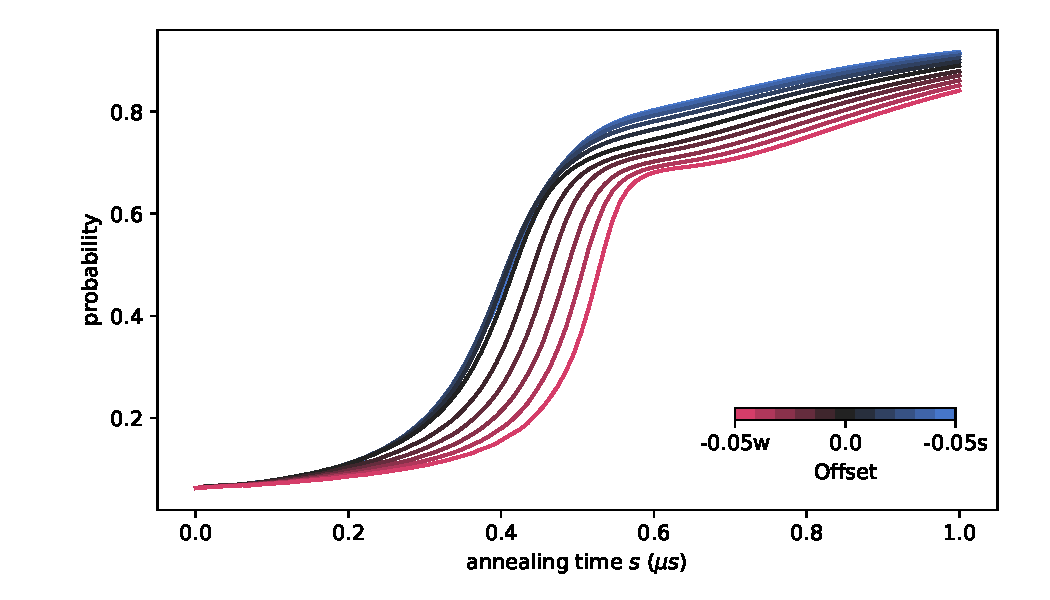
\includegraphics[width=\columnwidth]{./new_figures/time_dependent_probability.pdf}
	\caption{(Left) The time-dependent probability of resolving the ground state and (Right) the corresponding mutual information. (Top) Simulation with decoherence included and (Bottom) without decoherence.}
	\label{fig:td_prob}
\end{figure}

Finally, we comment that in order for the simulation to obtain the final state distribution shown in Fig.~\ref{fig:final_state_distribution}, effects of full-counting statistics are required. Absent some dynamical thermalization effect, the $G(2)$ problem is too small such that at a total annealing time of 1$\mu s$, the annealing offsets lift the ground state degeneracy by an amount such that diabatic transitions are absent, and the simulation is populated predominantly by the unique ground state. The final state distribution gives us a very sensitive observable to tune the simulation temperature, and agrees well with the experimental operating temperature.

\section{DATA AVAILABILITY}
	
Link to GitHub.

\section{ACKNOWLEDGEMENTS}

We thank x, y, z...

\section{AUTHOR CONTRIBUTIONS}

...

\section{ADDITIONAL INFORMATION}

\textbf{Competing Interests:} The authors declare no competing interests.

\bibliographystyle{naturemag-doi}
\bibliography{qilp}

\end{document}
